\documentclass[11pt,letterpaper]{article}
% Layout follows the SSAC "Paper Template": 1in sides, 1.1in top, 1.2in bottom,
% Cambria 11pt single spaced with 11pt after each paragraph, 42 Analytics logo bottom left.
\usepackage[left=1in,right=1in,top=1.1in,bottom=1.2in,footskip=0.3in]{geometry}
\usepackage[T1]{fontenc}
\usepackage{caladea}      % metric-compatible free clone of Cambria
\usepackage{amsmath}
\usepackage{amssymb}
\usepackage{booktabs}
\usepackage{float}
\usepackage[section]{placeins}
\usepackage{graphicx}
\graphicspath{{figs/}{./}}
\usepackage{xcolor}
\usepackage{tikz}
\usetikzlibrary{arrows.meta,positioning,fit,calc,shapes.geometric,backgrounds}
\usepackage[numbers]{natbib}
\setlength{\bibsep}{3pt}
\usepackage{titlesec}
\usepackage{fancyhdr}
\usepackage{eso-pic}
\usepackage{hyperref}
\hypersetup{colorlinks=true,linkcolor=black,citecolor=black,urlcolor=blue}

\setlength{\parindent}{0pt}
\setlength{\parskip}{11pt}
\titleformat{\section}{\fontsize{16}{19}\selectfont\bfseries}{\thesection.}{0.4em}{}
\titleformat{\subsection}{\fontsize{12}{14}\selectfont\bfseries}{\thesubsection.}{0.4em}{}
\titleformat{\paragraph}[runin]{\normalsize\bfseries}{}{0pt}{}
\titlespacing*{\section}{0pt}{6pt}{0pt}
\titlespacing*{\subsection}{0pt}{0pt}{-8pt}
\titlespacing*{\paragraph}{0pt}{0pt}{0.6em}
% after titlesec, which otherwise redefines \subsection and drops the barrier
\let\oldsubsection\subsection
\renewcommand\subsection{\FloatBarrier\oldsubsection}

\pagestyle{fancy}
\fancyhf{}
\renewcommand{\headrulewidth}{0pt}
\cfoot{\thepage}
\AddToShipoutPictureBG{\AtPageLowerLeft{\hspace*{0.9in}\raisebox{0.38in}{
\includegraphics[width=1.95in]{42analytics-logo.png}}}}

\newcommand{\papertitle}{Conditional Queries Against a Learned Hitter Process Model}
\newcommand{\papertrack}{Baseball}
\newcommand{\paperid}{Paper ID: 22}


\begin{document}
\raggedright
\thispagestyle{fancy}
\begin{center}
{\fontsize{18}{22}\selectfont\bfseries \papertitle\par}
\vspace{11pt}
{\fontsize{14}{17}\selectfont \papertrack\par \paperid\par}
\end{center}

\begin{center}{\fontsize{16}{19}\selectfont\bfseries Abstract}\end{center}
\vspace{-11pt}
In baseball, understanding how to use great hitters is often a simple task: play as many of them as you can and play them often. Teams try to gain an edge with the remaining hitters, but less playing time means thinner data in an area that takes hundreds of plate appearances to stabilize. This paper asks whether a model trained on pitches can project how a hitter will do against a type of matchup, like handedness or a specific pitching staff, with less data than standard projections need. We train a neural network inspired by (batter$|$pitcher)2vec that learns a 64-dimensional embedding for each of 1,672 hitters from 6.5 million Statcast pitches from 2015 through 2024, using only hitter-controlled pitch outcomes: swing decision, contact, exit velocity, launch angle, and spray direction. To query it, we reweight which pitchers the projection is drawn over and compose the outputs through the count-state Markov chain into a projected wOBA, so a new split needs a new weight vector, not a retrained model. The model is better at ordering hitters within a split than at predicting how many points of wOBA the split is worth. For a team, that makes it most useful for ranking platoon options among hitters with a moderate track record, where the decision is actually in question, not as a replacement for a projection system on raw accuracy. On 2025 wOBA against left- and right-handed pitchers, pooled RMSE was tied with gradient-boosted and empirical Bayes baselines (0.0433 against 0.0438 and 0.0444) and pooled rank correlation was higher (0.50 against 0.44 and 0.42). It beat both baselines on both measures only for hitters with 113 to 451 prior plate appearances, an exploratory result. With fewer than 113, its error was lower than both baselines' and its ranking margin over the boosted baseline was within noise. Hitters absent from the training seasons have no embedding and are not scored. Without being given definitions of power or contact, the embedding still separates hitters on both, with held-out accuracy of 0.79 and 0.75 against 0.33 by chance.


% =====================================================================================
\section{Introduction}
\label{sec:intro}

% Source: src/analysis/claim1_eval.py STABILIZATION_N_STAR = 226 (variance-components estimate,
% training seasons, hitters only).
Most lineup decisions are simple, because a team's best hitters play every day against every kind of pitcher. The decisions that leave room for an edge involve the bench and platoon hitters, and they usually depend on a split, which is how a hitter performs against one kind of pitcher. Examples include choosing which of two bench hitters starts against a left-handed pitcher and which pinch hitter to send up against the reliever warming up. Bench and platoon hitters are also the ones with the least data. In the training seasons, it takes about 226 plate appearances (PA) against left-handed pitchers before half of the variation in hitters' wOBA against them reflects skill rather than noise (Section~\ref{sec:eval}), and a part-time hitter can take several seasons to reach that many.

Much of that noise enters at the end of the plate appearance. Fielders, parks, and where a ball in play happens to land all change a plate appearance's wOBA value without reflecting anything the hitter did. The hitter's own contribution comes earlier and more often. On each pitch the hitter decides whether to swing, a swing either makes contact or misses, and Statcast records the exit velocity, launch angle, and direction of nearly every ball in play. A plate appearance lasts about four pitches and yields one wOBA value, but it yields several of these pitch-level outcomes, and they carry less of the luck that follows contact.

% Source: tango-2009 platoon constants note. The book page itself was never held; the constants
% are from Tango's 2009 comment quoting p.157, cited as such.
The usual way to project a split is to regress the observed split toward the league split for the hitter's batting side. In \citet[p.~157]{tango2007}, as quoted by one of its authors \citep{tango2009}, a right-handed hitter needs about 2,200 PA against left-handed pitchers before the observed split receives half the weight, and a left-handed hitter needs about 1,000. As a result, the estimate for most hitters stays close to the league-average split, and two part-time hitters from the same side receive nearly the same projection. This paper compares against an empirical Bayes version of that shrinkage \citep{efron1975} and against gradient-boosted trees \citep{chen2016} that add season summaries of each hitter's pitches.

\citet{alcorn2018} showed that a neural network can learn useful representations of players from their matchups alone. The (batter$|$pitcher)2vec model gave each batter and pitcher a nine-dimension embedding, trained to predict the outcome of each at-bat from the identities of the two players in Retrosheet data from 2013 through 2015. The embeddings grouped similar hitters without being told what made them similar, and they predicted outcome distributions for matchups absent from training better than simpler baselines. Alcorn suggested that predicting PITCHf/x measurements instead of discrete outcomes could convey more about players, and the model in this paper follows that suggestion with Statcast. Each hitter keeps a learned embedding, but the network predicts the hitter's response to each pitch from the pitch's measured characteristics, rather than the at-bat result from the pitcher's identity.

Later work took player embeddings in other directions. \citet{heaton2022} questioned whether one embedding should describe a player in every situation, and learned embeddings of a player's recent form from sequences of game events. \citet{heaton2023} used the same kind of sequence model to predict a player's strikeouts and hits in a single game. \citet{melville2023} paired a batter embedding with measured pitch characteristics to study pitch sequencing. This paper keeps one embedding per hitter and asks a different question of it, which is how the hitter projects against a chosen set of pitchers.

This paper makes three contributions. The first is a pitch-level hitter embedding model trained only on outcomes the hitter controls. The second is a query that turns the model into a projected wOBA against any weighted set of pitchers, so a new split needs new pitcher weights rather than a retrained model. The third is an evaluation against empirical Bayes and gradient-boosted baselines, grouped by how much history a hitter has against a hand and compared with the most that one season of outcomes can measure. On 2025 handedness splits, the model had higher pooled rank correlation than both baselines and beat both on error and rank correlation for hitters with a moderate track record. For hitters with little history against a hand, its error was lower than both baselines' and its ranking margin over the boosted baseline was within noise. It also learned recognizable traits such as power and contact from pitch outcomes alone.

% =====================================================================================
\section{Methods}
\label{sec:methods}

\subsection{Data}
\label{sec:data}

% Source: data/processed/phase_d5_clean_final/manifest.json; src/config/split_config*.json;
% decision log 2026-08-01, 2026-09-20.
Pitch-level Statcast data for the 2015 through 2025 regular seasons were pulled from Baseball Savant \citep{savant} with pybaseball \citep{pybaseball}. Each pitch carries its velocity, movement, release point, spin, plate location, pitch type, the count, and the handedness of both players, and each ball in play carries its exit velocity, launch angle, and a spray angle computed from where it was fielded \citep{albert2024}. Each plate appearance is valued in wOBA \citep{tango2007}, using each season's weights from FanGraphs \citep{fangraphsguts}. Bunts, pitchouts, automatic calls, pitches by position players or to pitchers batting, and pitches missing a core measurement were removed. The final data set consisted of 7,245,923 pitches. No minimum exposure was imposed, so every hitter in the training seasons has an embedding.

Model configurations were compared by training on 2015 through 2023 and scoring on 2024, the selection season. The chosen configuration was then retrained on 2015 through 2024, 6,540,616 pitches covering 1,672 hitters and 2,182 pitchers, and evaluated on 2025. Feature scaling was fit on 2015 through 2023 only, and the baselines saw only seasons before the one being scored.

\subsection{Model}
\label{sec:model}

% Source: paper/draft3/fig_arch.tex
\begin{figure}[!ht]
\centering
% fig_arch.tex -- architecture (a) and query (b) schematic. \input inside a figure env.
% needs: tikz with arrows.meta, positioning, fit, calc, shapes.geometric, backgrounds; amsmath; xcolor
\begin{tikzpicture}[
  x=1cm, y=1cm, font=\scriptsize, text=black!80, line width=0.5pt,
  box/.style={draw=black!55, rounded corners=1.5pt, align=center, inner sep=2pt,
              minimum height=0.5cm},
  acc/.style={draw=blue!60, fill=blue!7},
  bar/.style={draw=black!55, fill=black!5, rounded corners=1.5pt,
              minimum width=0.46cm, minimum height=5.6cm},
  head/.style={box, minimum width=3.2cm, anchor=west},
  arr/.style={-{Stealth[length=3.5pt,width=3pt]}, draw=black!60},
  cond/.style={-{Stealth[length=3pt,width=2.6pt]}, draw=blue!60, densely dashed},
  ttl/.style={anchor=west, font=\footnotesize\bfseries},
  note/.style={text=black!60},
  cnt/.style={draw=black!45, rounded corners=1pt, inner sep=0pt, minimum width=0.42cm,
              minimum height=0.26cm, font=\tiny},
  stepc/.style={circle, draw=blue!60, fill=blue!7, inner sep=0pt, minimum size=0.38cm,
                font=\scriptsize\bfseries},
  para/.style={anchor=north west, align=left, inner sep=0pt},
]

% ---------------------------------------------------------------- (a) the network
\node[ttl] at (0,8.55) {(a) The network};

\node[box, acc, minimum width=2.45cm] (hid) at (1.25,7.55) {Hitter ID $h$};
\node[box, acc, minimum width=2.45cm] (emb) at (1.25,6.65) {Embedding (64)};
\node[box, minimum width=2.45cm, text width=2.3cm] (ctx) at (1.25,4.9)
  {Pitch context (46)\\[1pt]{\tiny\color{black!60}physical measurements,
   location, type, handedness of both players, count}};
\node[box, minimum width=2.45cm] (c1) at (1.25,3.45) {Context layer (128)};
\node[box, minimum width=2.45cm] (c2) at (1.25,2.55) {Context layer (128)};
\draw[arr] (hid) -- (emb);
\draw[arr] (ctx) -- (c1);
\draw[arr] (c1) -- (c2);

\node[bar] (cat) at (3.05,5.0) {};
\node[bar] (t1)  at (3.8,5.0)  {};
\node[bar] (t2)  at (4.55,5.0) {};
\node[rotate=90] at (cat) {Concatenate (64 + 128)};
\node[rotate=90] at (t1)  {Trunk layer (256)};
\node[rotate=90] at (t2)  {Trunk layer (256)};
\draw[arr] (emb.east) -- (cat.west |- emb.east);
\draw[arr] (c2.east)  -- (cat.west |- c2.east);
\draw[arr] (cat) -- (t1);
\draw[arr] (t1) -- (t2);

% six heads, top to bottom in plate-appearance order
\foreach \name/\y/\lbl in {
    sw/7.45/{Swing},
    co/6.47/{Contact $\mid$ swing},
    sp/5.49/{Foul/tip/in play $\mid$ contact},
    ev/4.51/{Exit velocity {\color{black!60}(24 bins)}},
    la/3.53/{Launch angle $\mid$ EV {\color{black!60}(24)}},
    sy/2.55/{Spray $\mid$ EV, LA {\color{black!60}(24)}}} {
  \node[head] (\name) at (5.1,\y) {\lbl};
  \draw[arr] (t2.east |- \name.west) -- (\name.west);
}
% EV and LA bins feed the later heads
\draw[cond] (ev.east) to[out=0, in=0, looseness=1.3] (la.east);
\draw[cond] (ev.east) to[out=0, in=0, looseness=1.1] (sy.east);
\draw[cond] (la.east) to[out=0, in=0, looseness=1.3] (sy.east);

\node[box, dashed, draw=black!50, text width=8.1cm, inner sep=3pt] (take) at (4.25,1.3)
  {Take table, fit separately and not part of the network\\[1pt]
   $p(\text{ball},\ \text{called strike},\ \text{HBP} \mid
     \text{location, batter hand, pitcher hand})$};

% panel divider
\draw[black!20] (8.85,0.8) -- (8.85,8.7);

% ---------------------------------------------------------------- (b) a query
\begin{scope}[xshift=9.15cm]
\node[ttl] at (0,8.55) {(b) A query};

% step 1
\node[stepc] (s1) at (0.2,7.9) {1};
\node[para, text width=6.4cm] at (0.55,8.03)
  {For pitcher $j$ and each count, sample 6 of the pitcher's real pitches in that count
   to same-side hitters. Run the network for hitter $h$ and average.\\[3pt]
   {\color{blue!60}$\Rightarrow$} per count $p_B$, $p_S$, $p_F$, $p_H$ and $v(b,s)$,
   the expected wOBA from a ball in play\\(its chance times its average value)};

% step 2, the 12-count chain
\node[stepc] (s2) at (0.2,5.5) {2};
\begin{scope}[shift={(0.95,5.5)}]
  \foreach \b in {0,...,3} \foreach \s in {0,1,2}
    \node[cnt] (n\b\s) at (0.62*\b,-0.48*\s) {\b-\s};
  \foreach \b in {0,1,2} \foreach \s in {0,1,2} {
    \pgfmathtruncatemacro{\nb}{\b+1}
    \draw[arr, draw=black!40] (n\b\s) -- (n\nb\s);}
  \foreach \b in {0,...,3} \foreach \s in {0,1} {
    \pgfmathtruncatemacro{\ns}{\s+1}
    \draw[arr, draw=black!40] (n\b\s) -- (n\b\ns);}
  \node[cnt, acc] at (n00) {0-0};
  \node[note, font=\tiny, anchor=south] at ($(n10.north)!0.5!(n20.north)+(0,0.03)$)
    {balls $\rightarrow$};
  \node[note, font=\tiny, anchor=north] at (n12.south |- 0,-1.15) {strikes $\downarrow$};
\end{scope}
\node[para, text width=3.45cm] at (3.3,5.63)
  {Count-state Markov chain over the 12 counts, solved backward from the end states\\[3pt]
   {\color{blue!60}$\Rightarrow$} $W_{hj} = W(0,0)$};

% step 3
\node[stepc] (s3) at (0.2,3.45) {3};
\node[para, text width=6.4cm] at (0.55,3.58)
  {Weighted mean over the pitcher set $S$, with weights proportional to batters faced};
\node[anchor=west] at (0.5,2.42)
  {$\widehat{\text{wOBA}}_S(h)=\sum_j w^S_j\, W_{hj}, \qquad
    w^S_j\propto \text{BF}_j\,\mathbf{1}[j\in S]$};
\node[box, draw=blue!60, text width=6.2cm, inner sep=3pt, anchor=north west]
  at (0.55,1.98) {A new split is a new set $S$, so only the weights change.
                 No retraining.};

\draw[arr] (s1) -- (s2);
\draw[arr] (s2) -- (s3);
\end{scope}
\end{tikzpicture}

\caption{(a) The hitter's embedding and the pitch context feed a shared trunk, and six heads predict the hitter-controlled outcomes of the pitch. (b) Outcomes against one pitcher are composed through the count into $W_{hj}$, and a weighted average over the chosen pitchers gives the projection.}
\label{fig:arch}
\end{figure}

% Source: src/model/v1.py heads; data manifest n_quality_bins 24; decision log 2026-08-08.
The model architecture can be seen in Figure~\ref{fig:arch}a. Each hitter has a 64-dimension embedding, a learned vector that is the only input identifying the hitter. The same embedding covers all training seasons, and a projection describes the hitter across those seasons together. Each pitch is described by a 46-dimension context vector built from its physical measurements, location, type, the handedness of both players, and the count. The pitcher enters only through the pitches thrown, not through an identifier, which lets the model describe any pitcher whose pitches it has seen. Because the count is the only game state included, predictions reflect the hitter and the pitch rather than the game situation.

The context passes through two fully connected layers of 128 units, each followed by a ReLU activation, and is then joined with the hitter's embedding in a shared trunk of two more such layers of 256 units. Each layer builds features out of the layer before it. The first context layer turns the raw pitch measurements into features, and the second combines them, for example location with count. The first trunk layer is where the hitter and the pitch first meet, and the second builds on those combinations, which lets one hitter respond differently from another to a combination of pitch features such as a high fastball with two strikes. Six heads read the trunk in the order a plate appearance unfolds. The first three give the probability of a swing, the probability of contact given a swing, and whether contact is a foul, a foul tip, or a ball in play (a two-strike foul tip is a strikeout and a foul is not). The other three give the exit velocity, launch angle, and spray direction of a ball in play, each in 24 bins. Launch angle is predicted given exit velocity, and spray given both, so the three are never treated as independent.

Taken pitches are modeled as depending on the pitcher and the umpire rather than the hitter. Their outcomes therefore come from a table fit on the training seasons, which gives the probability of a ball, a called strike, or a hit batter for each plate location and pairing of batter and pitcher hand, as in the called-strike model of \citet{deshpande2017}.

% Source: src/model/v1.py loss; src/model/train.py masks.
The network is trained to maximize the summed log-likelihood of each hitter's outcomes,
\begin{equation}
\begin{split}
\mathcal{L} = \sum_{i} \Big[ & \log p(a_i) + m^{c}_i \log p(c_i) + m^{t}_i \log p(t_i \mid c_i) + m^{e}_i \log p(e_i) \\
& + m^{l}_i \log p(l_i \mid e_i) + m^{s}_i \log p(s_i \mid e_i, l_i) \Big],
\end{split}
\label{eq:loss}
\end{equation}
where for pitch $i$, $a_i$ is the swing decision, $c_i$ the contact outcome, $t_i$ the contact type (foul, foul tip, or ball in play), and $e_i$, $l_i$, and $s_i$ the exit velocity, launch angle, and spray bins. Every probability is conditioned on the hitter $h$ and the pitch context $x_i$. Each mask $m_i$ is one when the outcome exists and was measured, so contact is scored only on swings, contact type only on contact, and the three quality terms only on measured balls in play.

% Source: results/model_v1/sweep_log.csv (dim64 1.02327 vs dim32 1.02378; lr1e3 1.02584/1.02585 vs
% lr1e3_warm2k 1.02564/1.02596); decision log 2026-09-02/03 (SGD table, lr 1.0), 2026-09-04
% (cold-start prior -0.00077 [-0.00119,-0.00020], rank 0); RPS screen (1.19715 vs 1.07582);
% checkpoint clean_dim64_final_s0.pt (266,317 parameters).
The network has 266,317 parameters. Weights outside the embedding table are trained with AdamW \citep{loshchilov2019} at a learning rate of $10^{-3}$, batches of 8,192 pitches, weight decay of $10^{-2}$, and dropout of 0.1 in the trunk. The embedding table is trained with plain stochastic gradient descent at a learning rate of 1.0, because an adaptive optimizer would give a rarely seen hitter steps as large as a regular's, while plain gradient descent moves each embedding in proportion to the hitter's data \citep{stollenwerk2025}. The 64-dimension embedding was chosen over 32 because it gave the lower 2024 log loss.\footnote{Three other choices were checked on 2024. Training the quality heads on a ranked probability score instead of log likelihood fit clearly worse. A 2,000-step learning-rate warmup changed mean log loss by less than 0.0001. Giving hitters absent from training the average embedding of low-exposure hitters from their side, rather than an untrained vector, lowered their RMSE by 0.0008 and left rank correlation unchanged, and it is used for all results.} Five copies are trained from different seeds as a deep ensemble \citep{lakshminarayanan2017}, and each head's predicted distribution is averaged across the five. The model was implemented in PyTorch, and each copy trains on a CPU in about 25 minutes. The code will be released publicly, and the link is withheld here for anonymous review.

\subsection{Querying the model}
\label{sec:query}

% Source: src/model/query.py docstring; src/model/query_tables.py; decision log 2026-08-08.
The network describes a single pitch, while a lineup decision concerns many plate appearances against many pitchers. A query takes a hitter, a set of pitchers, and a weight for each pitcher, and returns the hitter's projected wOBA per plate appearance against those pitchers. It connects the single pitch to the decision in three steps (Figure~\ref{fig:arch}b).

The first step fixes one pitcher. For pitcher $j$ and each count, the network is run for hitter $h$ on a sample of real pitches that $j$ threw in that count to hitters from $h$'s side, and the outputs are averaged. This gives, for each count, the probability that the pitch ends as a ball, a strike, a foul, a hit batter, or a ball in play. A ball in play is valued at the league's average wOBA for its exit velocity, launch angle, and spray bins, weighted by the hitter's predicted probability of each combination, so its value sets aside the fielder and park effects described in Section~\ref{sec:intro}, as xwOBA does \citep{mlbxwoba}. Unmeasured balls in play, about 8\%, take the league's average value.

The second step plays out the plate appearance. Each pitch moves the count to a new state or ends the plate appearance, so the expected wOBA from any count is a sum over the possible pitch outcomes. Each term is the probability of that outcome times the expected wOBA of the count or result it leads to. The count moves as a Markov chain over 12 states from 0-0 to 3-2 \citep{powers2025}, and the expected wOBA from count $(b,s)$ satisfies
\begin{equation}
W(b,s) = p_B\, W(b+1,s) + p_S\, W(b,s+1) + p_F\, W(b,\min(s+1,2)) + p_H\, w_{\text{HBP}} + v(b,s),
\label{eq:chain}
\end{equation}
where $p_B$, $p_S$, $p_F$, and $p_H$ are the probabilities of a ball, a strike, a foul, and a hit batter in that count, $v(b,s)$ is the expected value from a ball in play, a fourth ball is worth a walk's wOBA weight, and a third strike is worth zero. A two-strike foul leaves the count unchanged, and that loop is solved directly. Working back from the terminal states gives $W_{hj} = W(0,0)$, the projected wOBA of hitter $h$ in one plate appearance against pitcher $j$, with no simulation.

The third step chooses the pitchers. The projection is the hitter's expected wOBA if every plate appearance came against the chosen set of pitchers $S$, each in proportion to the batters that pitcher faced in the training seasons, $\text{BF}_j$,
\begin{equation}
\widehat{\text{wOBA}}_S(h) = \sum_{j} w^S_j \, W_{hj}, \qquad w^S_j \propto \text{BF}_j \, \mathbf{1}[j \in S].
\label{eq:query}
\end{equation}
A platoon split takes $S$ as all left-handed or all right-handed pitchers. Any set of pitchers the model has seen can be queried without retraining, and the weights need not be batters faced (Section~\ref{sec:otherqueries}). Each projection also carries a nominal 95\% interval built from the spread of the five seeds and the sampling noise of the plate appearances being projected.

\subsection{Evaluation}
\label{sec:eval}

% Source: src/analysis/claim1_eval.py:95-108 (n* 226, CI [199, 264], cuts (113, 452), floor 10 PA);
% baseline_ladder_bivariate_eb.py (3 trailing seasons); paired CSV (2,000 batter-clustered draws).
The handedness query is scored on units, where a unit is one hitter's wOBA against one pitcher hand in 2025 with at least 10 PA. Units are limited to hitters who appear in the training seasons. A hitter who does not has no embedding, and the model gives every such hitter the same projection for a batting side and pitcher hand. Results are reported for all units and by prior exposure, the hitter's PA against that hand in all earlier seasons since 2015. Reliability is the share of the variation between hitters that is not sampling noise \citep{franks2016}. For wOBA against left-handed pitchers after $n$ PA it is $n/(n+n^*)$, which reaches one half at $n^* = 226$ PA in the training seasons (95\% interval 199 to 264). Units fall into three strata, low (fewer than 113 prior PA), medium (113 to 451), and high (452 or more), with cuts at half and twice $n^*$.

The empirical Bayes baseline takes a hitter's wOBA against each hand over the previous three seasons and shrinks the two sides jointly toward the league average for the hitter's batting side, with the correlation between sides estimated from the data. The boosted baseline is fit on one row per hitter, season, and pitcher hand, using the same trailing outcomes plus the hitter's pitch summaries by pitcher hand and pitch group. Each method is scored by root mean squared error (RMSE) and by Spearman rank correlation, both weighted by each unit's 2025 PA. Differences between the model and a baseline carry 95\% intervals from 2,000 bootstrap draws that resample batters.

% =====================================================================================
\section{Results}
\label{sec:results}
\label{sec:test}

% Source: model_v1_claim1_scores_min_pa_sweep_clean_dim64_final.csv; paired CSV; verdict JSON;
% results/paper_draft3/seen_only_rescore.csv (population "all" reproduces Table 1 and the min-PA sweep at floors 10 and 50).
The 2025 results by prior exposure can be seen in Table~\ref{tab:test} and Figure~\ref{fig:strata}. The low stratum was specified in advance as the test. There (220 units, 153 batters) the model's RMSE is 0.0588 against 0.0617 for the boosted baseline and 0.0630 for empirical Bayes, with differences of $-0.0029$ (interval $-0.0053$ to $-0.0005$) and $-0.0043$ ($-0.0070$ to $-0.0016$). Its rank correlation is 0.23 against 0.17 and 0.11. That interval excludes zero against empirical Bayes (0.002 to 0.258) but not against the boosted baseline ($-0.070$ to 0.188). At a 50 PA floor the RMSE difference against the boosted baseline is $-0.0041$ ($-0.0072$ to $-0.0012$). Analysis of the other strata was exploratory.

\begin{table}[!ht]
\centering\small
\begin{tabular}{lrrrrrrr}
\toprule
 & & \multicolumn{3}{c}{RMSE (lower better)} & \multicolumn{3}{c}{Rank corr. (higher better)} \\
\cmidrule(lr){3-5}\cmidrule(lr){6-8}
Prior PA & Units & Model & GBM & EB & Model & GBM & EB \\
\midrule
Low & 220 & 0.0588 & 0.0617 & 0.0630 & 0.23 & 0.17 & 0.11 \\
Medium & 280 & 0.0455 & 0.0479 & 0.0492 & 0.42 & 0.28 & 0.22 \\
High & 493 & 0.0395 & 0.0385 & 0.0387 & 0.50 & 0.49 & 0.48 \\
All & 993 & 0.0433 & 0.0438 & 0.0444 & 0.50 & 0.44 & 0.42 \\\bottomrule
\end{tabular}
\caption{2025 side-specific wOBA by prior PA against the hand, for hitters seen in the training seasons. GBM is the gradient-boosted baseline and EB empirical Bayes.}
\label{tab:test}
\end{table}

Across all 993 units the model's RMSE is 0.0433 against 0.0438 for the boosted baseline and 0.0444 for empirical Bayes, and both difference intervals include zero. Its weighted rank correlation is 0.50 against 0.44 and 0.42, and those intervals, 0.012 to 0.096 and 0.026 to 0.127, exclude zero. In the medium stratum the model beats both baselines on both measures, with all four intervals excluding zero. Its rank correlation is 0.42 against 0.28 for the boosted baseline and 0.22 for empirical Bayes, and its RMSE is about 2 points of wOBA below the boosted baseline and 4 below empirical Bayes. In the high stratum the three methods are even.

\begin{figure}[!ht]
\centering
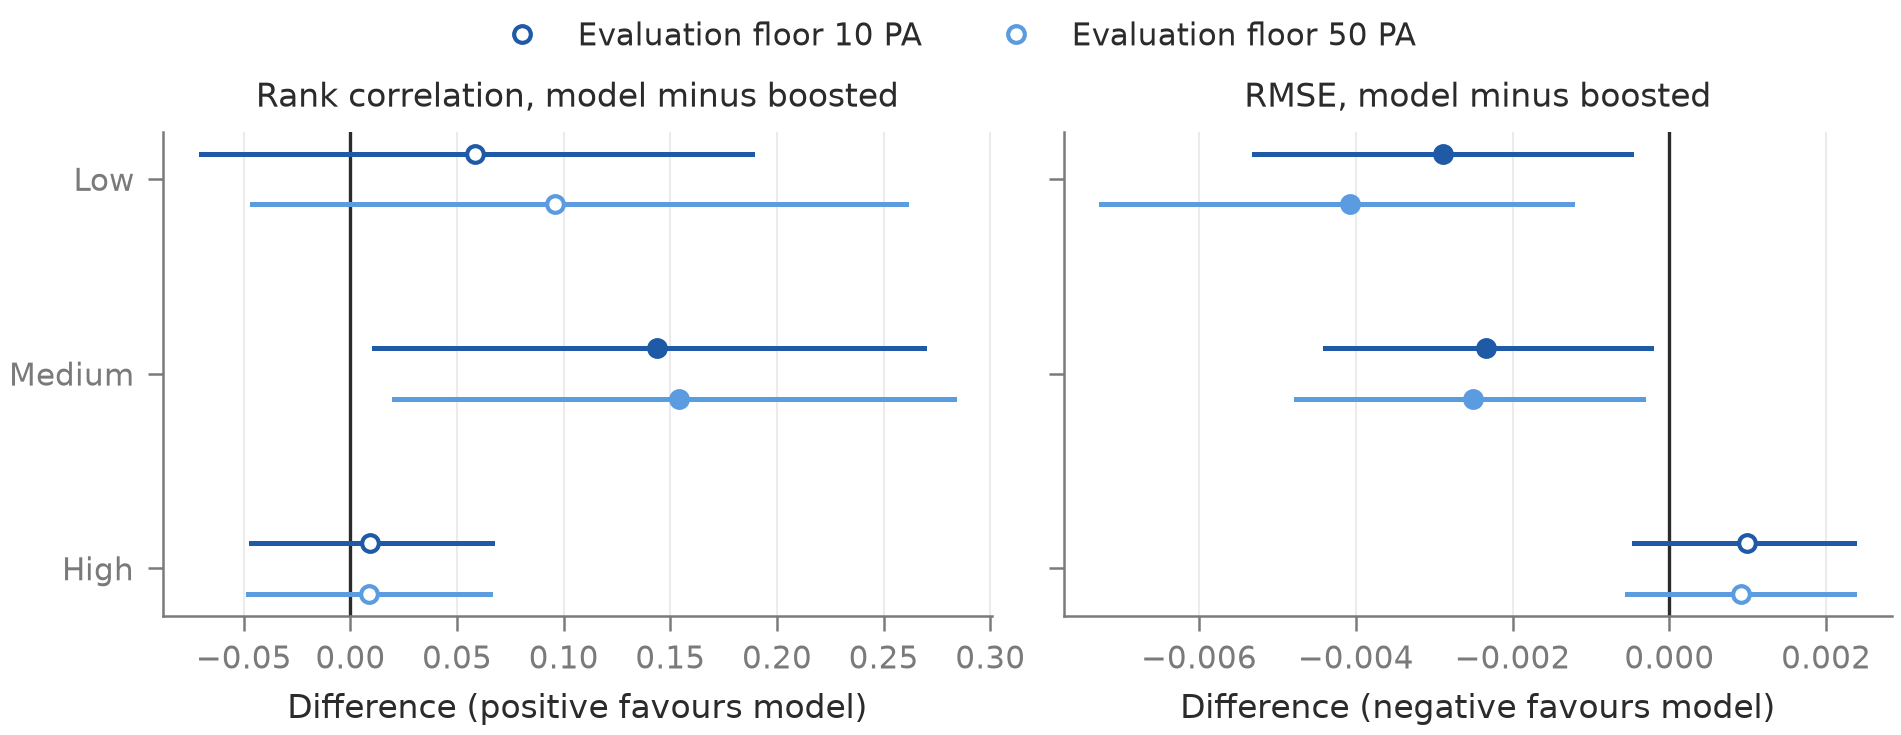
\includegraphics[width=0.72\linewidth]{fig_strata_seen.png}
\caption{The model's 2025 margin over the boosted baseline on rank correlation and error by stratum, at evaluation floors of 10 and 50 PA, with 95\% intervals. A filled marker means the interval excludes zero in the model's favour. Raising the floor from 10 to 50 PA changes no row's outcome.}
\label{fig:strata}
\end{figure}

% Source: results/v_chain_clean/paper_figures/fig_calibration_2025 source JSON;
% coverage_labels_coverage_labels.csv (coverage 0.8642, 987 units);
% results/paper_draft3/seen_only_calibration.csv (seen-only low slope 0.8428, se 0.1769, pred 0.2939 vs obs 0.2896).
A PA-weighted regression of each unit's observed 2025 wOBA on its projection gives a slope of 0.98 in the medium stratum, 0.93 in the high, and 0.84 in the low (Figure~\ref{fig:calibration}). Across all strata the slope is 0.89, below one by about two standard errors. High-stratum projections averaged about 9 points of wOBA above the observed values and low-stratum projections about 4 points above. On 2024, the nominal 95\% intervals covered the observed value for 86\% of 987 units. Nearly all of their width comes from the sampling noise of the plate appearances, and the seed spread alone has a mean half-width of about 6 points.

\begin{figure}[!ht]
\centering
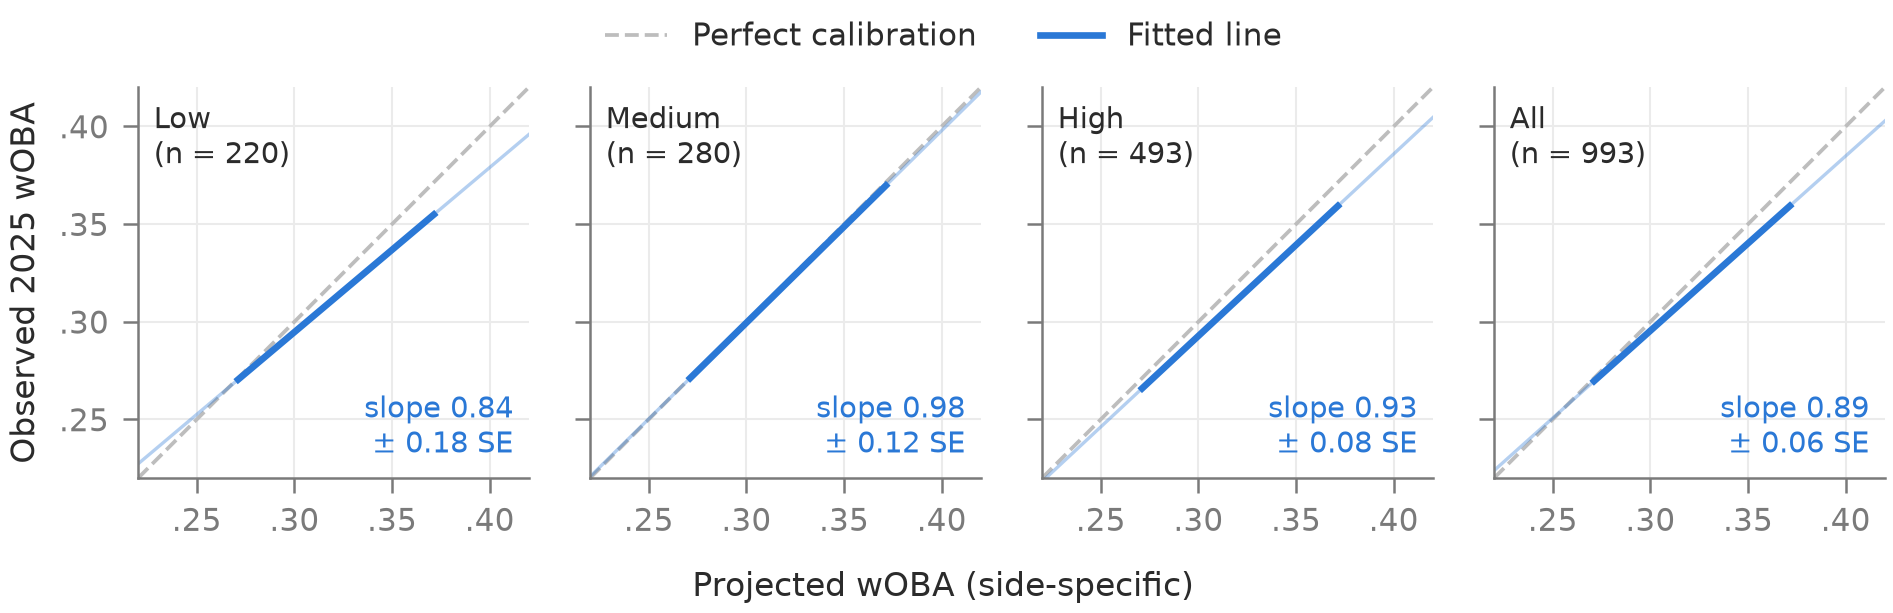
\includegraphics[width=0.95\linewidth]{fig_calibration_seen.png}
\caption{Calibration of 2025 side-specific projections by stratum, as the PA-weighted regression of observed on projected wOBA, The dashed diagonal is perfect calibration.}
\label{fig:calibration}
\end{figure}

% Source: results/case_studies_2025/case_studies_2025.json (468, 255/213, wmae 0.0438 / 0.0452);
% all_hitters_bootstrap.json (diff 0.0015 [0.0002, 0.0027], share [0.500, 0.590]).
% Regenerate: scripts/seen_only_2025_frame.sh
Graded against each hitter's observed 2025 platoon split, the model's projected split was closer than the empirical Bayes projection for 255 of the 468 hitters with at least 10 PA against each hand (54\%, interval 50\% to 59\%). Weighted by the harmonic mean of each hitter's PA against the two hands, its mean absolute error was 0.0438 against 0.0452, a difference of 0.0015 (interval 0.0002 to 0.0027).

\subsection{How much signal one season holds}
\label{sec:ceiling}

% Source: results/measurement_ceiling_clean/differential_fraction_of_ceiling.csv (0.3066);
% differential_exhibit.csv (0.1788, EB 0.1470, GBM 0.1516; RMSE 0.0612 vs floor 0.0615);
% level_ceiling_level_ceiling.json (0.754, 0.482); differential_fraction_of_ceiling.csv (fraction CI 0.242-0.898).
One season of outcomes limits how well any projection can score. The share of the spread in hitters' observed values that is not sampling noise is the reliability of Section~\ref{sec:eval}. Because noise in the observed values weakens any correlation with them \citep{spearman1904}, reliability sets the highest rank correlation any method could reach. On 2024, the selection season, for the 473 hitters with at least 10 PA against each hand, that ceiling is 0.754 for a hitter's level, and the model reaches 0.482, or 64\% of it (Figure~\ref{fig:ceiling}). For the platoon split, after removing each batting side's average split, the ceiling is about 0.31. The model reaches 0.179, or 58\% (interval 24\% to 90\%), against 48\% for empirical Bayes and 49\% for the boosted baseline. The model's RMSE for the split is 0.0612, close to the 0.0615 floor that sampling noise sets, the error a projection that knew each hitter's true skill would still make \citep{brown2008}, and empirical Bayes is about as close.

\begin{figure}[!ht]
\centering
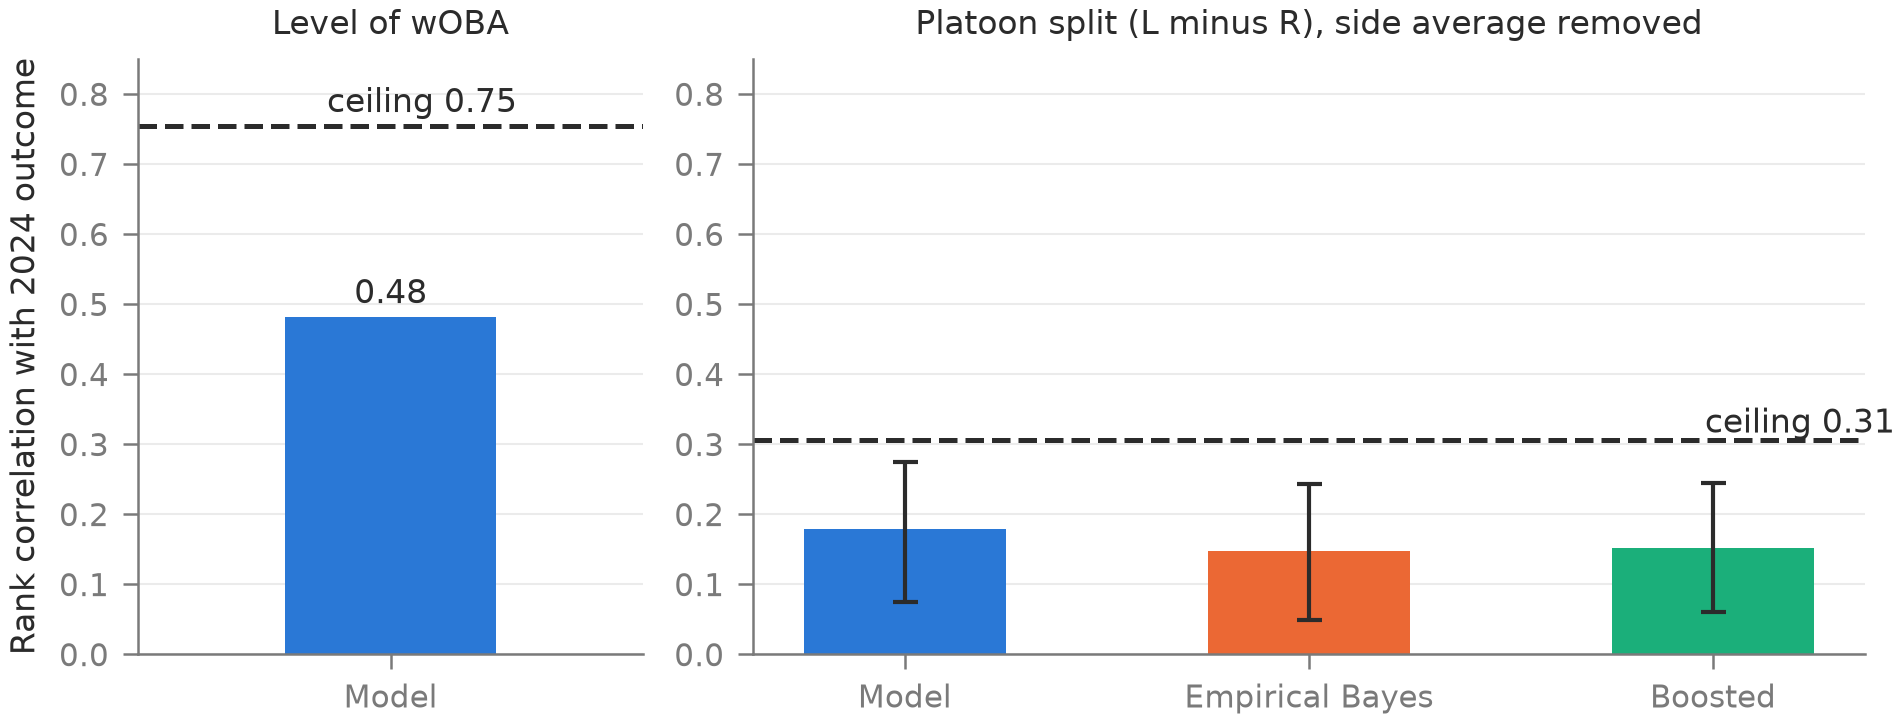
\includegraphics[width=0.85\linewidth]{fig_ceiling_seen.png}
\caption{Rank correlation with 2024 outcomes against the ceiling one season allows (dashed), for the level of wOBA (left) and the platoon split after removing each batting side's average (right). Bars are 473 hitters with at least 10 PA against each hand, and the split bars carry 95\% intervals from resampling hitters.}
\label{fig:ceiling}
\end{figure}
% =====================================================================================
\section{Discussion}
\label{sec:discussion}\label{sec:ordering}

% Source: Section 3 numbers; seen_only_rescore.csv.
The model is better at saying which of two hitters will do better against a hand than at saying by how many points. Empirical Bayes sits just as close to the error floor for the split (Section~\ref{sec:ceiling}), so one season of outcomes cannot show much skill at sizing a split for any method, and the model's nominal 95\% intervals covered only 86\% of outcomes. Many lineup decisions depend only on order. Choosing which of two bench hitters starts against a left-handed pitcher is a ranking question, and a few points of error in both projections do not change the call if the two are in the right order.

The model's advantage varies with exposure. With heavy exposure, several seasons of outcomes already measure a hitter well, which leaves little for any method to add. With moderate exposure, a hitter has seen enough pitches from a hand for the embedding to describe how the hitter handles them, while the outcomes of those plate appearances are still too few to stabilize, and this is where the clearest gain appears. With little exposure the model's error is still lower than both baselines', but its ordering is not clearly better than the boosted baseline's. Each projection is also made against the training seasons' pitchers of a hand, weighted by batters faced, not against the pitchers the hitter actually met in 2025, so part of every error reflects the schedule rather than the hitter. For a team, the model is most useful for ranking platoon options among hitters with some track record.

\subsection{What the model learned}
\label{sec:embedding}

% Source: results/v_chain_clean/embedding_structure/embedding_structure.json; embedding_alt_views.json
% (LDA 5-fold, n 1,493, power 0.791, contact 0.754, zone swing 0.746, chase 0.734);
% seed_stability_corrected_null.json (0.837 vs 0.123). Selection model (trained through 2023).
The loss scores single pitches and never sees a hitter-level statistic, so any such summary in the embedding was assembled by the model. The analyses here use the selection model, trained through 2023, with each hitter's embedding averaged over the five seeds and scaled to unit length.\footnote{The five seeds give similar vectors for the same hitter, with a median cosine similarity of 0.84 after rotating each onto the first, against 0.12 when hitters are shuffled before the rotation is fit. Embeddings are averaged after this alignment. They are scaled to unit length because an embedding's length grows with the hitter's exposure (correlation 0.93 with log prior PA), and after scaling the main direction of variation is nearly unrelated to playing time (0.09).} A linear classifier on the embedding recovers a hitter's power third (90th-percentile exit velocity) for 79\% of 1,493 hitters and contact third (contact rate on swings) for 75\%, against 33\% by chance, and in-zone swing rate (75\%) and chase rate (73\%) nearly as well. Placed on the fitted power and contact directions, hitters' observed wOBA rises toward high power and high contact (Figure~\ref{fig:powercontact}).

\begin{figure}[!ht]
\centering
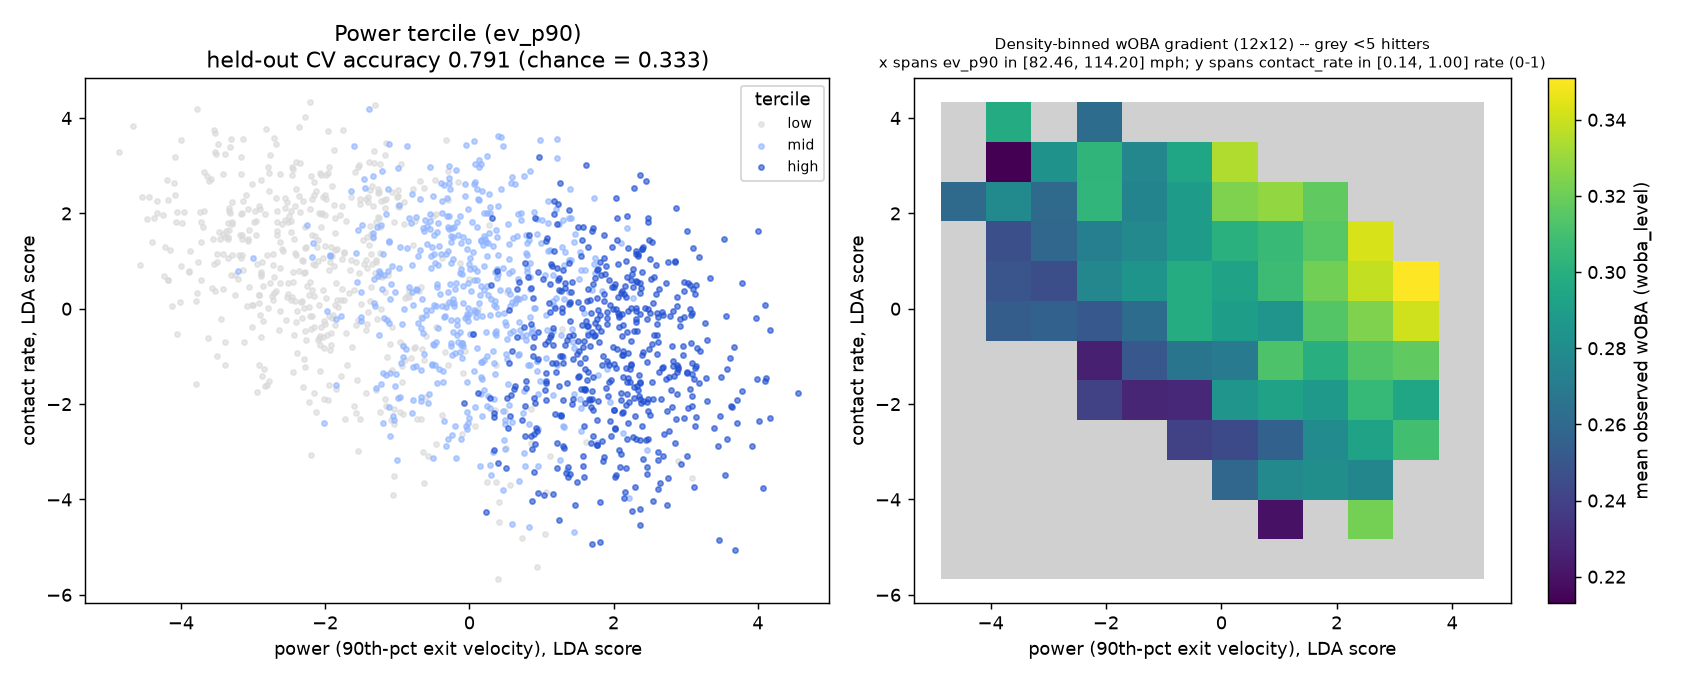
\includegraphics[width=0.95\linewidth]{fig1_power_contact.png}
\caption{Hitters placed by the embedding on fitted power and contact directions, colored by observed power tercile (left) and by mean observed wOBA per cell (right).}
\label{fig:powercontact}
\end{figure}

% Source: make_figs3.py fig_miss_damage (asserts match to embedding_alt_views.json).
The embedding separates some skills by pitch type and not others (Figure~\ref{fig:missdamage}). Directions fit to whiff rate on breaking balls and on fastballs correlate at 0.64 across hitters, and many hitters rank much worse against one pitch family than the other, as their observed whiff rates do (0.53). Directions fit to power on the two families correlate at 0.94, against 0.83 observed, so the model treats power as close to a single skill and whiffing as partly specific to the pitch, which is how the data behave.

\begin{figure}[!ht]
\centering
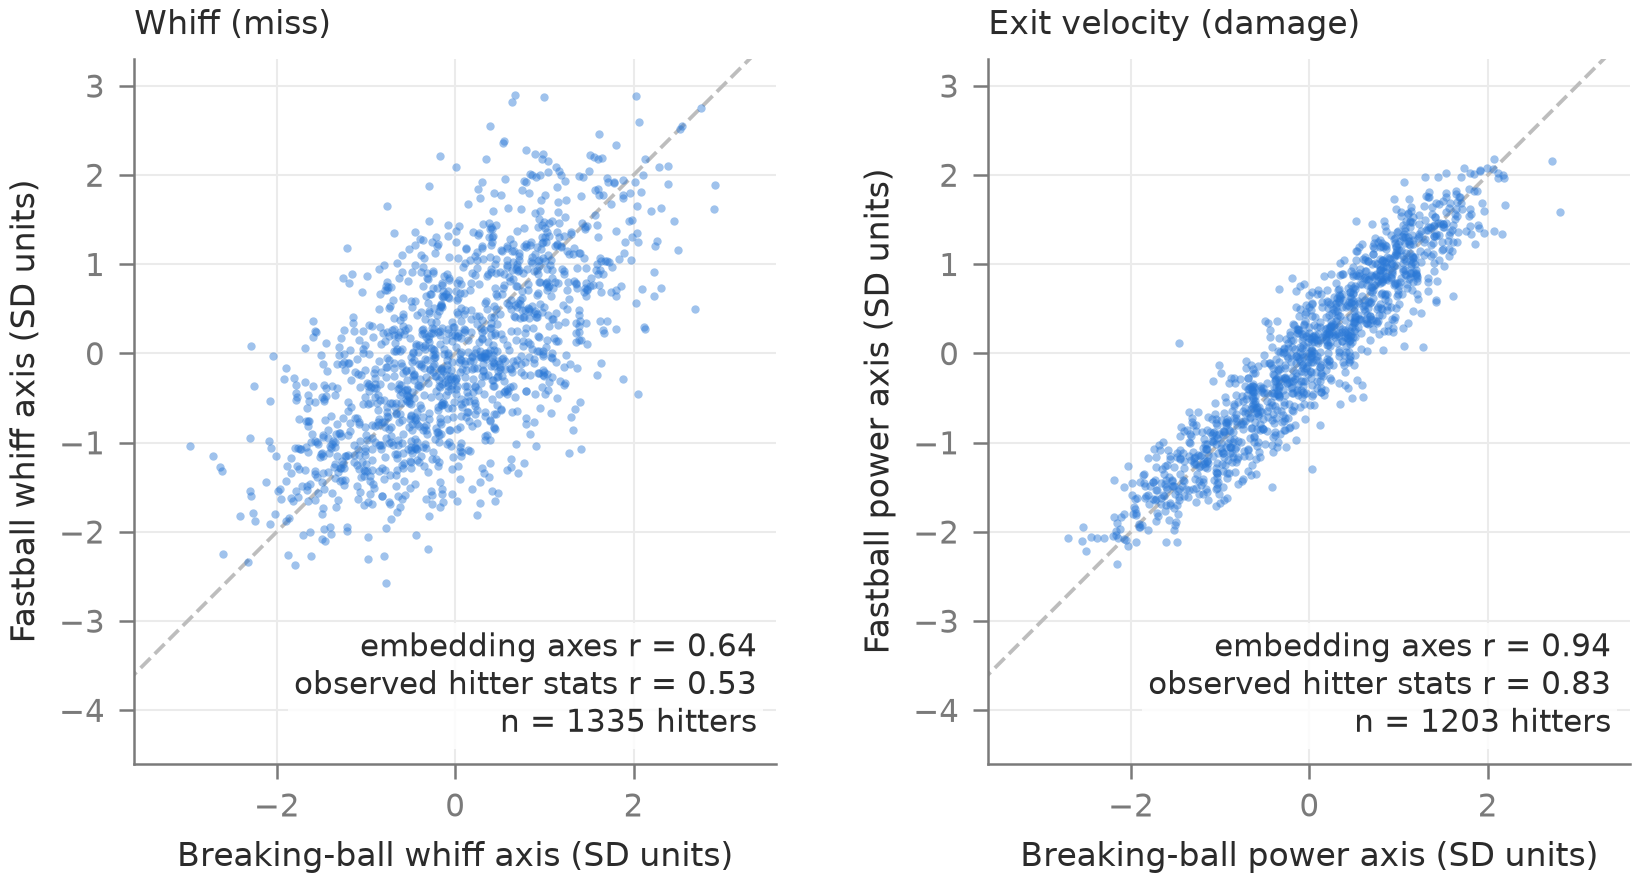
\includegraphics[width=0.8\linewidth]{fig_miss_damage.png}
\caption{Hitters placed on embedding directions fit to breaking-ball and fastball whiff rate (left, 1,335 hitters) and power (right, 1,203 hitters), in standard deviations. The dashed line is equal standing on both pitch families.}
\label{fig:missdamage}
\end{figure}

% Source: results/v_chain_clean/fig_head_partial_heatmap source.
Each head also follows the standard statistic for its own part of the plate appearance (Figure~\ref{fig:headpartial}). Averaged over a fixed set of 2,000 training-season pitches and with log prior PA removed, the swing head's output tracks a hitter's swing rate (0.67), the contact head whiff rate ($-0.56$), the exit velocity head bat speed (0.61, for 570 hitters with bat tracking), and the launch angle and spray heads average launch angle (0.49) and pull rate (0.34).

\begin{figure}[!ht]
\centering
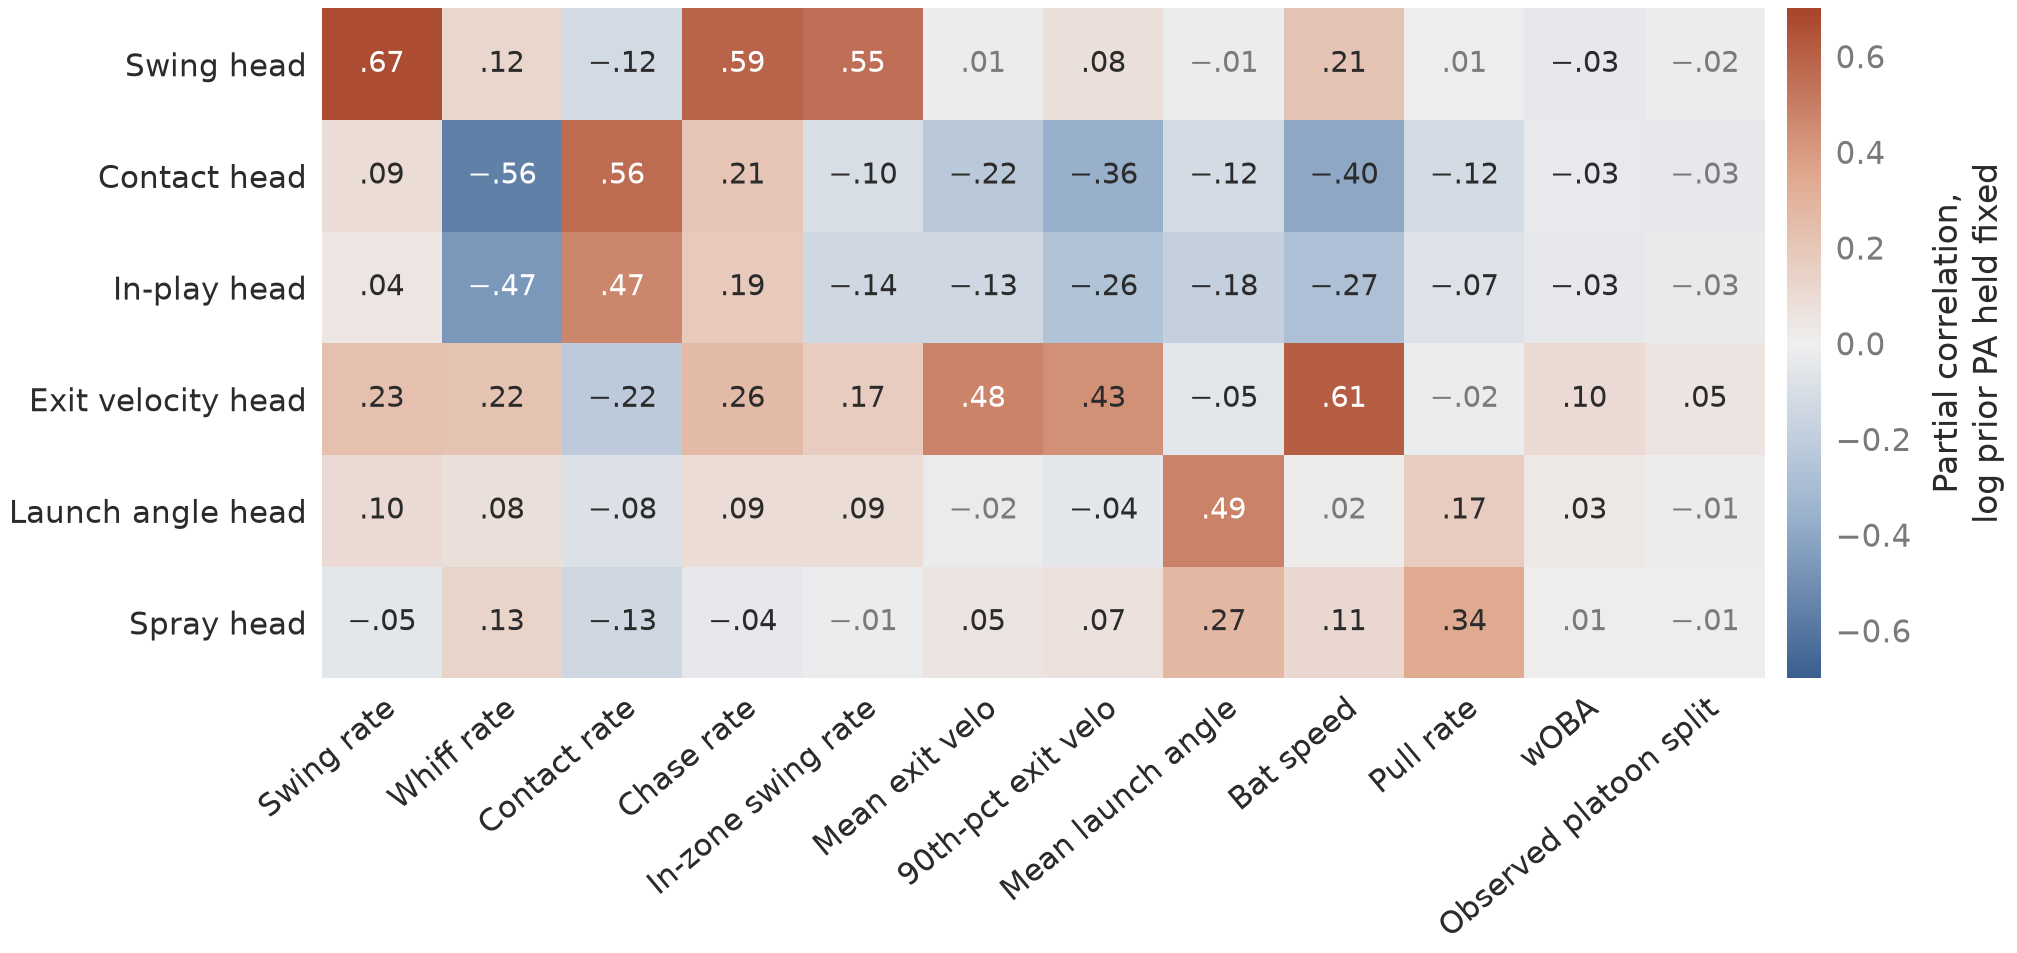
\includegraphics[width=0.78\linewidth]{fig_head_partial.png}
\caption{Correlation between each head's hitter-specific output and observed hitter statistics in the training seasons, after removing log prior PA.}
\label{fig:headpartial}
\end{figure}

% Source: v_chain_clean/paper_figures/platoon_sign_agreement.json (262/473, null 0.497); platoon/platoon_projection.json
% (cosine 0.142 [0.081, 0.201], partial r 0.074 / 0.144 / 0.133).
The platoon split is held more weakly. After removing each batting side's average split, the model's projected 2024 split has the same sign as the observed split for 262 of 473 hitters (55\%), against 50\% when hitters are shuffled. The direction in the embedding along which the projected split grows has a cosine of only 0.14 (interval 0.08 to 0.20) with a direction fit to the empirical Bayes split. A hitter's position along it correlates with the observed training-season split at 0.07 in the low stratum, 0.14 in the medium, and 0.13 in the high, each with an interval above zero. The split is a faint direction in the embedding, and it is faintest for the hitters with the least history.

\subsection{Nearest neighbors}
\label{sec:neighbors}

% Source: results/paper_draft3/neighbours_seed_mean_high.csv (seed-mean embedding, high stratum;
% 7/40 overlap); embedding_structure/neighbour_purity.csv (0.57 vs 0.33); silhouette max 0.054.
Nearest neighbors in the embedding show what the model treats as similar. Among high-exposure hitters, Joc Pederson's closest neighbor is Kyle Schwarber, followed by Paul Goldschmidt, Rafael Devers, Joey Gallo, Kendrys Morales, Josh Donaldson, Mark Trumbo, and Pete Alonso, power hitters from both sides of the plate. Schwarber's closest is Pederson. Juan Soto's list includes Max Muncy, Shin-Soo Choo, José Bautista, and Andrew McCutchen, and Alec Bohm's includes Bo Bichette, Ryan Mountcastle, Tommy Edman, and Ian Desmond, with none of the sluggers on Pederson's list. Mike Trout's neighbors are Ronald Acuña, Eugenio Suárez, Pete Alonso, Austin Jackson, Jake Lamb, Brandon Belt, Anthony Rendon, and Denard Span. Ranked instead by ten observed statistics covering plate discipline, contact quality, and wOBA, Trout's nearest are Yordan Álvarez, Goldschmidt, Soto, Mookie Betts, Joey Votto, Rhys Hoskins, Acuña, and Will Smith, and only Acuña is on both lists. Across these five hitters the two kinds of list share 7 of 40 names, so the embedding's similarity is not a restatement of season statistics.

A hitter's ten nearest neighbors share the hitter's power third 57\% of the time, against 33\% with shuffled labels, but the silhouette score is at most 0.054 for any number of clusters from two to ten. The space holds neighborhoods of similar hitters rather than a set of distinct hitter types.

\subsection{Case studies}
\label{sec:anchors}\label{sec:disagree}

% Source: results/case_studies_2025/case_studies_2025.{csv,json}; v_chain_clean/disagreement_summary.json,
% disagreement_top.csv (2024 projections, seed 0 of the selection model).
Table~\ref{tab:cases} gives the projected 2025 splits for five well-known hitters. Pederson and Schwarber, left-handed hitters, project worse against left-handed pitchers. Bohm, a right-handed hitter, projects better against them, and Trout projects close to flat. Soto, an everyday player, projects 0.041 worse against left-handed pitchers, and Soto's observed 2025 split ran the same way. Empirical Bayes tells the same story for all five and was slightly closer in 2025 for each, by 0.002 to 0.014, but no observed split is more than 1.96 standard errors from the midpoint of the two projections. Pederson shows how wide that noise is. With 19 PA against left-handed pitchers, Pederson's observed split of $+0.172$ has a standard error of 0.121, wide enough to include either projection and zero.

\begin{table}[!ht]
\centering\small
\begin{tabular}{llrrrr}
\toprule
Hitter & Bats & Model & EB & Observed (SE) & $z$ \\
\midrule
Joc Pederson & L & $-0.047$ & $-0.039$ & $+0.172$ (0.121) & 1.77 \\
Kyle Schwarber & L & $-0.042$ & $-0.028$ & $+0.025$ (0.039) & 1.52 \\
Juan Soto & L & $-0.041$ & $-0.044$ & $-0.074$ (0.041) & 0.78 \\
Mike Trout & R & $+0.009$ & $+0.007$ & $-0.062$ (0.056) & 1.25 \\
Alec Bohm & R & $+0.022$ & $+0.033$ & $+0.042$ (0.052) & 0.28 \\
\midrule
Aaron Judge & R & $+0.020$ & $+0.003$ & $+0.038$ (0.049) & 0.54 \\
José Altuve & R & $+0.021$ & $+0.026$ & $+0.013$ (0.051) & 0.22 \\
Marcell Ozuna & R & $+0.020$ & $+0.002$ & $-0.006$ (0.050) & 0.33 \\
\bottomrule
\end{tabular}
\caption{2025 platoon split (wOBA against left-handed minus right-handed pitchers) for five well-known hitters (top) and three of the ten on whom the model and empirical Bayes disagreed most in 2024 (bottom). $z$ is the observed split's distance from the midpoint of the two projections in standard errors.}
\label{tab:cases}
\end{table}

The two methods disagree most where pitch-level information pulls a projection away from a hitter's outcome history. Their 2024 projected splits have a rank correlation of 0.77 overall, and 0.69 for high-exposure hitters, where empirical Bayes shrinks least. Ranked within batting side, Robbie Grossman has the largest split among right-handed hitters by empirical Bayes and only the 283rd by the model. Marcell Ozuna is the reverse, 6th by the model and 275th by empirical Bayes, and the model also ranks Aaron Judge and José Altuve much higher. In 2025 the observed splits of Judge and Altuve fell closer to the model's projection and Ozuna's closer to empirical Bayes, each within about half a standard error of the midpoint. The evidence on split accuracy is the aggregate comparison in Section~\ref{sec:results}.

\subsection{Other queries}
\label{sec:otherqueries}

% Source: results/v_chain_clean/surfaces_location.csv (selection model clean_clean_dim64, seed 0);
% make_figs3.py fig_surfaces_obs. Observed rows and the two correlations:
% results/v_chain_clean/surfaces_location_observed.csv and surfaces_location_agreement.json,
% from src/analysis/surfaces_observed.py.
Because the network scores single pitches, any set of pitches or pitchers defines a query, and only the handedness query was graded here. One alternative is a set of pitch locations. Figure~\ref{fig:surfaces} shows each case-study hitter's expected wOBA on a ball in play by location, relative to the average of 100 hitters on the same pitches. Schwarber and Soto do their best damage on pitches in the upper middle of the zone, up to about 170 points above average, and Soto falls below average on low pitches. Trout's best results come on low pitches over the middle, about 200 to 220 points above average. Bohm's surface is nearly flat, about 30 to 40 points above average at the median, with no cell above about 70. Each surface changes little between pitcher hands. The observed rows of the figure show the same quantity computed from each hitter's measured balls in play in the training seasons, 2015 to 2023, in cells with at least 20 balls in play. Across those 116 cells the model and observed values have a correlation of 0.54. In 2024, which the model was not trained on, the correlation is 0.61 across the 26 cells with at least 20 balls in play.

\begin{figure}[!ht]
\centering
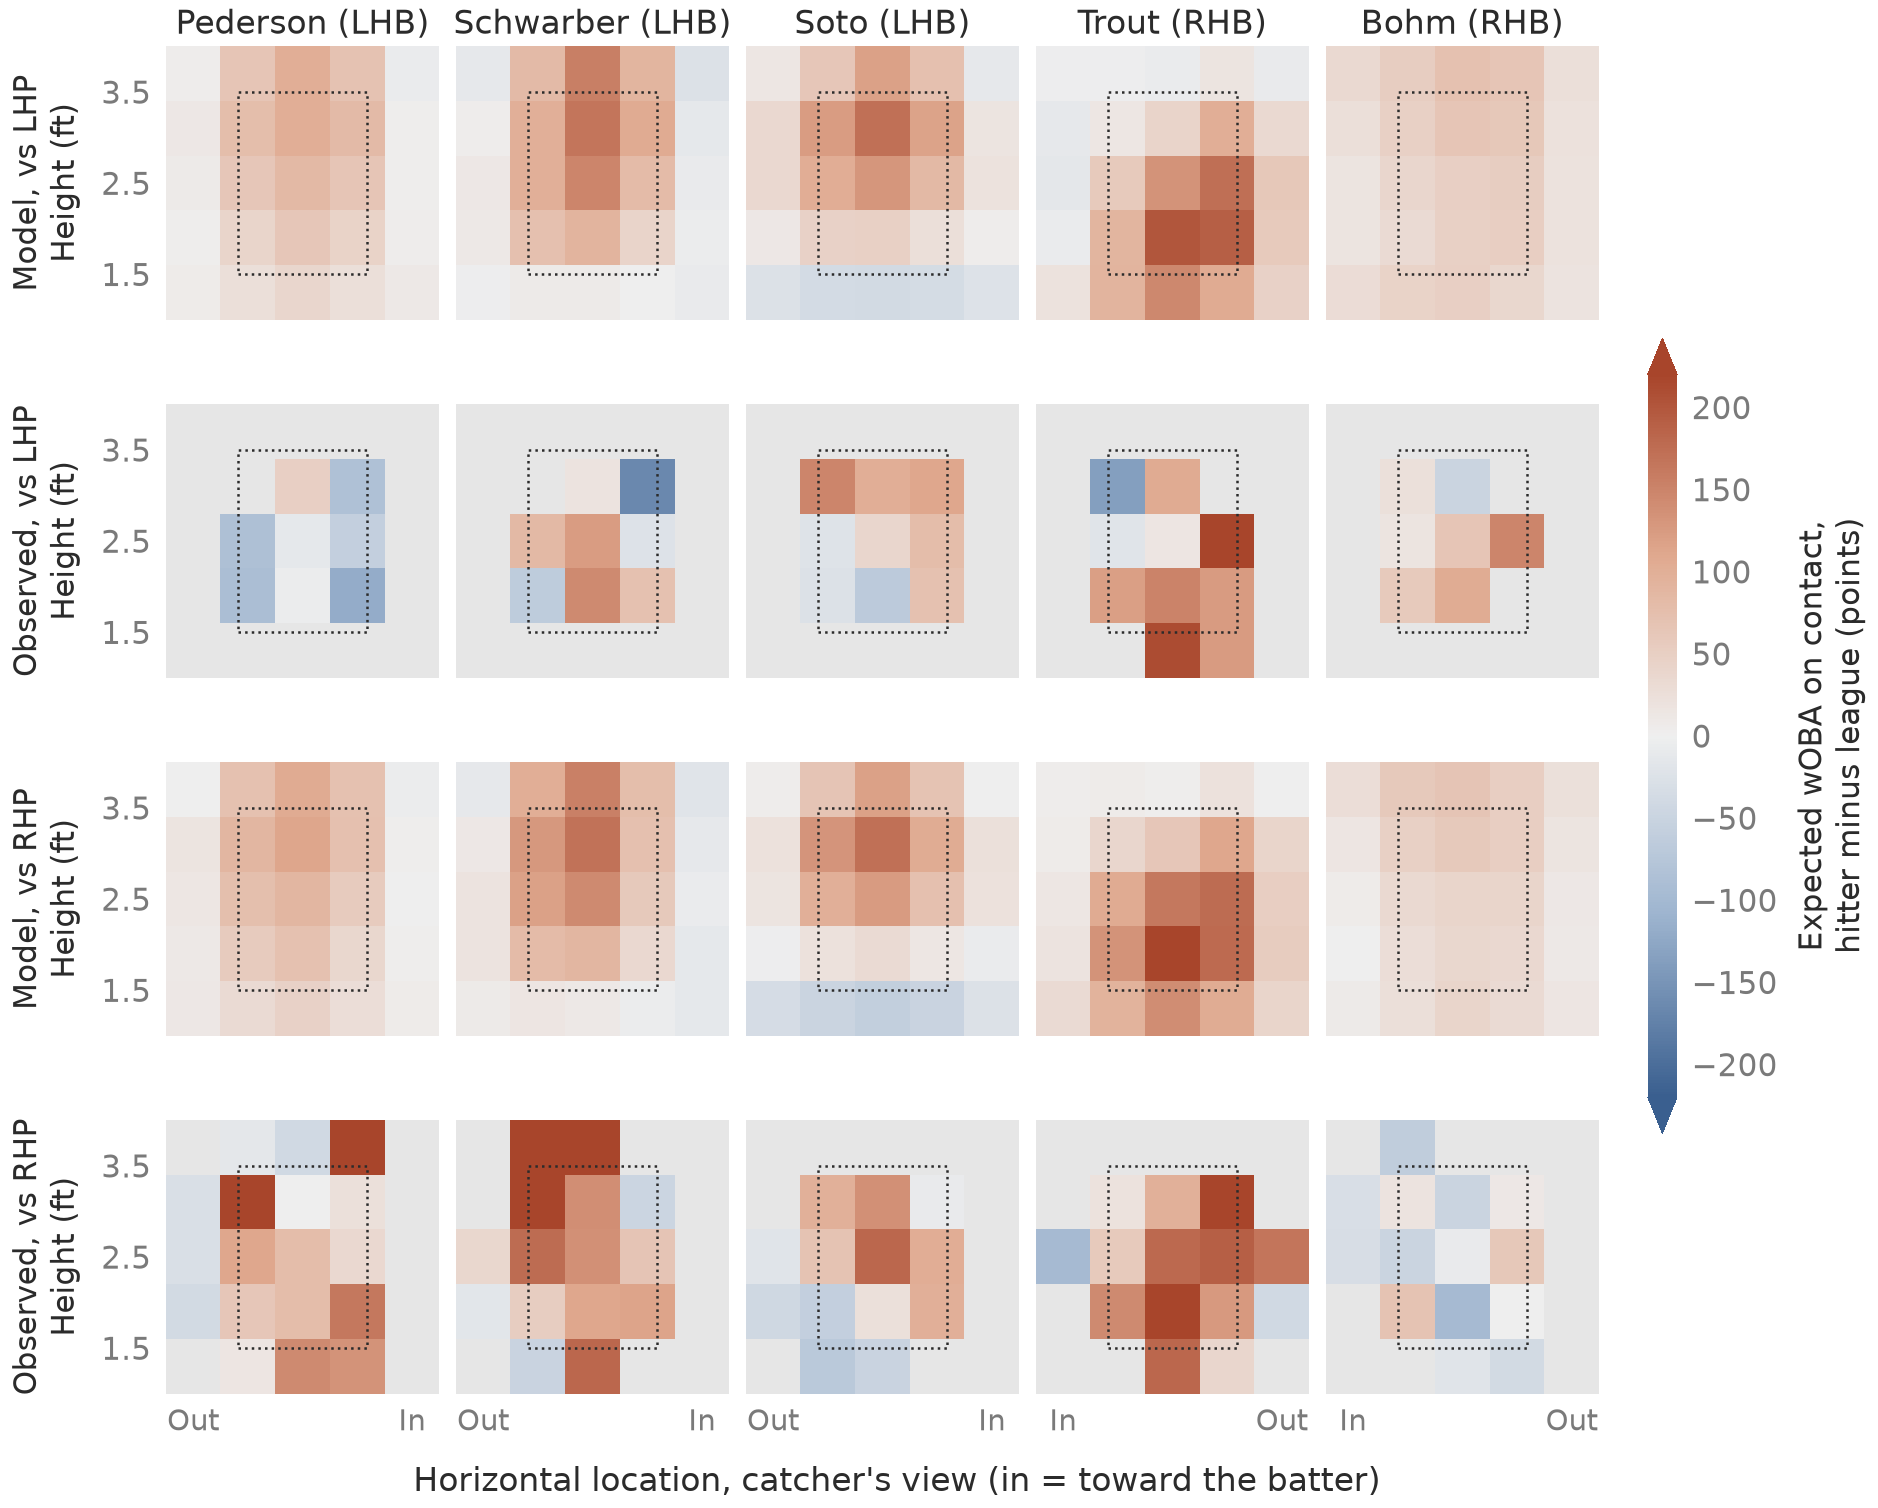
\includegraphics[width=\linewidth]{fig_surfaces_obs.png}
\caption{Expected wOBA on a ball in play by pitch location, from the catcher's view, against left-handed (top two rows) and right-handed (bottom two rows) pitchers. Model rows are the hitter minus the average of 100 hitters on the same pitches. Observed rows are the hitter's measured balls in play in 2015 to 2023, which are training seasons, minus all hitters in the same cell; grey cells have fewer than 20 balls in play. The dotted box is the strike zone.}
\label{fig:surfaces}
\end{figure}

% Source: src/analysis/paper_single_game_staff.py -> results/paper_draft3/single_game_staff{.csv,.json,
% _weights.csv}. Final model, five-seed ensemble; generic projections match the cached final run.
% EB and GBM columns: same script, baseline_vs_lhp() (projections only, built as in the scored 2025 run).
A query can also target one game. For the Phillies' game against the Braves on August 30, 2025, with Chris Sale starting, the opposing staff was weighted as Sale's average of 25.1 batters faced per start in the training seasons plus Atlanta's average of 14.9 relief batters faced per game. The relief share was split among the 16 relievers who had pitched for Atlanta in the previous 30 days, in proportion to their 2025 relief batters faced. A rule dropping relievers who had pitched on both previous days or thrown 25 or more pitches the day before removed none. One reliever the model cannot query, carrying 0.2\% of the weight, was left out. Table~\ref{tab:staff} ranks the 13 Phillies who started a game within four days of this one. Against this staff every hitter projects 7 to 35 points below their generic projection against left-handed pitchers, with Brandon Marsh dropping most, but the order barely moves and only three adjacent pairs swap. The model's top nine are eight of the nine Phillies who started that day, with Max Kepler in place of Edmundo Sosa. The two baselines can only be asked about left-handed pitchers in general. Their top nine are the same as each other's and also include eight of the nine starters, with Rafael Marchán in place of Harrison Bader, so the model and the baselines disagree on two of the nine places. The query ignores defense, positions, and rest, so the ranking is one input to a lineup rather than a lineup.

\begin{table}[!ht]
\centering\small
\begin{tabular}{lcrrrrrr}
\toprule
 & & \multicolumn{2}{c}{Projected wOBA} & \multicolumn{2}{c}{Model rank} & \multicolumn{2}{c}{Baseline rank} \\
\cmidrule(lr){3-4}\cmidrule(lr){5-6}\cmidrule(lr){7-8}
Hitter & Started & vs staff & vs LHP & vs staff & vs LHP & EB & GBM \\
\midrule
Alec Bohm & \checkmark & 0.332 & 0.357 & 1 & 1 & 3 & 2 \\
Trea Turner & \checkmark & 0.327 & 0.341 & 2 & 3 & 2 & 4 \\
Bryce Harper & \checkmark & 0.324 & 0.341 & 3 & 2 & 1 & 1 \\
J. T. Realmuto & \checkmark & 0.322 & 0.339 & 4 & 4 & 4 & 5 \\
Nick Castellanos & \checkmark & 0.307 & 0.334 & 5 & 5 & 6 & 7 \\
Kyle Schwarber & \checkmark & 0.302 & 0.327 & 6 & 6 & 7 & 3 \\
Max Kepler & & 0.299 & 0.320 & 7 & 7 & 11 & 10 \\
Harrison Bader & \checkmark & 0.292 & 0.306 & 8 & 8 & 10 & 12 \\
Weston Wilson & \checkmark & 0.283 & 0.304 & 9 & 9 & 5 & 6 \\
Edmundo Sosa & \checkmark & 0.279 & 0.291 & 10 & 11 & 9 & 9 \\
Bryson Stott & & 0.273 & 0.293 & 11 & 10 & 12 & 11 \\
Rafael Marchán & & 0.271 & 0.278 & 12 & 13 & 8 & 8 \\
Brandon Marsh & & 0.251 & 0.286 & 13 & 12 & 13 & 13 \\
\bottomrule
\end{tabular}
\caption{Phillies hitters projected against the Braves' staff for August 30, 2025 (Sale starting, bullpen weighted by recent use) and against all left-handed pitchers. The baseline ranks are against all left-handed pitchers. Started marks the actual lineup.}
\label{tab:staff}
\end{table}
% =====================================================================================
\section{Future directions}
\label{sec:future}

% Source: results/model_evaluation_final_clean/model_v1_claim1_verdict_min_pa_sweep_clean_dim64_final.json
% (rank_power: medium 377 needed, x1.60 = 236 batters; low seen-only 1,532 needed, x10.01 = 153 batters, power_restatement on seen_only_rescore.csv).
The most direct application is a matchup card that ranks a team's options against a pitcher hand or a projected staff, as in Section~\ref{sec:otherqueries}, with a band around each projection. The same query could compare a trade or free-agent target with the hitters already on the roster against the pitchers a team expects to face, a single-split version of the roster comparison \citet{alcorn2018} proposed for player embeddings. Before a card can show a band, the prediction intervals need recalibrating. The moderate-exposure advantage was found in exploratory analysis and should be tested on 2026 and later seasons. Detecting it at its 2025 size with 80\% power would take about 377 batters, against 236 batters (280 units) in the 2025 medium stratum, so 2026 may need to be pooled with later seasons. Confirming the low-exposure ranking margin at its observed size would take about 1,500 batters, roughly 10 times the 153 batters in that stratum.

Hitters absent from training now receive one generic projection per batting side and pitcher hand, and they are left out of the evaluation. A prior built from what is known about a new hitter, or minor league data mapped into the same space as \citet{alcorn2018} suggested, could give them a better starting point. Other weightings of $S$, such as the single reliever warming up, pitchers grouped by arm angle, or pitchers grouped by pitch mix, need held-out targets and baselines of their own before they can inform decisions.

% =====================================================================================
\section{Conclusion}
\label{sec:conclusion}

This paper trained a hitter embedding on pitch outcomes the hitter controls and queried it for a projected wOBA against a chosen set of pitchers. On 2025 handedness splits, among hitters seen in training, the model tied both baselines on error and ordered hitters better overall. It beat both baselines on both measures only for hitters with 113 to 451 prior PA against the hand, an exploratory result that needs a new season to confirm. With fewer prior PA its error was lower than both baselines'. The model is better at ordering hitters within a split than at sizing the split, so its use for a team is ranking platoon options among hitters with a moderate track record. Because a query is only a set of pitcher weights, the same model can be asked about a staff or a set of pitch locations without retraining, and each of those queries still needs its own test.

\bibliographystyle{plainnat}
\bibliography{refs}

\end{document}
